\subsection{Connections}\label{sec:mit-connections}

As mentioned in \vref{sec:mit-address}, each address comes with a protocol where the protocol represents a connection type as presented in \vref{fig:mit-protocol-map}.

\begin{figure}
\centering
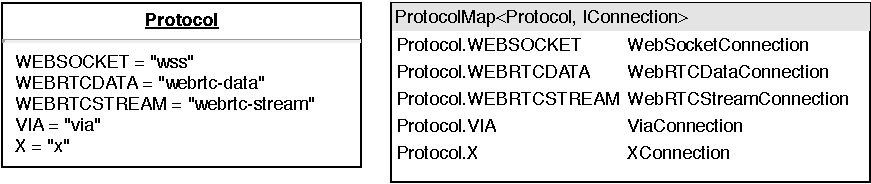
\includegraphics[width=0.75\textwidth]{graphics/implementation/mitosis-architecture-connections-protocol-map.pdf}
\caption{Protocol Map}
\label{fig:mit-protocol-map}
\end{figure}

By extending the \lstinline|ProtocolMap| other connection types can be supported. For example, when a future release shall support Bluetooth, a new entry can be added in the \lstinline|Protocol| definition and mapped to the concrete implementation in the \lstinline|ProtocolMap|.

\begin{figure}
\centering
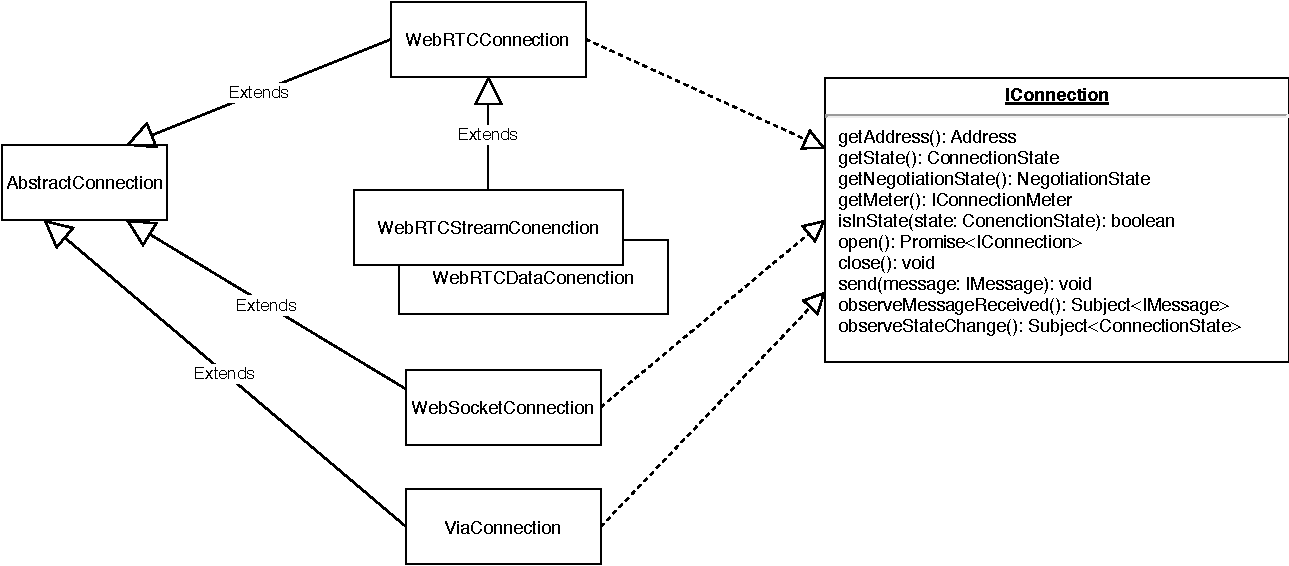
\includegraphics[width=1\textwidth]{graphics/implementation/mitosis-architecture-connections.pdf}
\caption{Connections}
\label{fig:mit-connections-uml}
\end{figure}

\vref{fig:mit-connections-uml} shows how connections are designed.

The interface specifies the methods that each connection has to implement. As some logic can be handled in a general way, an abstract connection is available. Every connection has to implement the interface but can optionally choose to extend the abstract connection class.

Common functionality a connection has to provide, includes the opening process and sending of messages. The WebRTC connection, for example, has to implement the negotiation process as explained in \vref{sec:webrtc-con-negotiation}.
